\documentclass[conference]{IEEEtran}
\usepackage{graphicx}
\begin{document}
\title{Word Hunter}
\author{\IEEEauthorblockN{Yang Zhao}
\IEEEauthorblockA{yzhao3@stanford.edu}
\and
\IEEEauthorblockN{Shuo Liu}
\IEEEauthorblockA{shuol@stanford.edu}
\and
\IEEEauthorblockN{Lingren Zhang}
\IEEEauthorblockA{lz7@stanford.edu}
}

% make the title area
\maketitle


\begin{abstract}
For this project we propose and implement a reading tool on Andriod platform that can be used to identify keywords on paper-based media.  After receiving an image of the media, we first pre-process the image (binarization and de-skew), and then use OCR (in particular, Tesseract OCR engine) to recognize the text and find the keywords, at last we highlight the keywords by circling it with a red box.
\end{abstract}

\section{Introduction}
Have you ever read a long paper-based article and find yourself unable to locate keywords? With the advancement of digital media, sometimes we take basic word search for granted. But the world is still full of media printed on paper and it would make our lives much simpler if we can automate this basic reading tool for good old fashioned books. We propose a mobile application that will be able to find a word that the user specified through a phone’s viewfinder. As soon as the phone detects the word it will highlight it, saving the user many minutes of looking for the word him/herself. 

For example, we want to search for “nonlinear equation” in this page of paper. We only need to use our smart phone to scan over the paper. Whenever the word “nonlinear equation” appears on the phone screen, it will be immediately circled in red.\\

\begin{figure}
\center
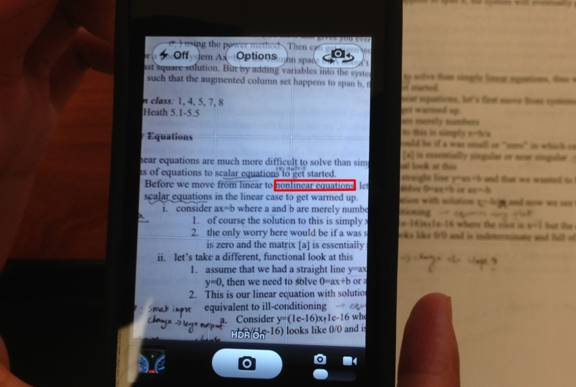
\includegraphics[scale=0.5]{demo.jpg}
\caption{Word Hunter Demo}
\end{figure}

\section{Preprocessing}
\subsection{Binarization}

The first step is to apply locally adaptive thresholding algorithm in order to separate text from background in a grayscale image (which can be derived from RGB).  The reason we choose locally adaptive thresholding instead of global thresholding is that the lighting/brightness of the image is not uniform which will cause global thresholding to perform poorly in the extreme bright/dark regions.

The idea of locally adaptive thresholding is divide the image into blocks/windows.  For each block, use grayscale variance to determine whether the block is uniform.  If the block is non-uniform (high variance), apply Otsu's method/global thresholding to the block; if the block is uniform (low variance), classify the entire block as all black or all white based on the mean grayscale value.  The reason not to apply Otsu's method to every block is because some blocks maybe entirely background with a number of noise pixels, Ostu's method will keep the noise pixels while classifying the entire block as background will eliminate noise.

We applied OpenCV function adaptiveThreshold for binarization.  We also observed that a blockSize of 51 yields the best thresholding result.  See Figure~\ref{noskew} and Figure~\ref{noskewbinarized} for an example of image before and after binarization.

We also performed, as part of the binarization step, a median filtering with a kernel size of 3 to eliminate any salt-and-pepper noise.  This will improve the accuracy of the character size detection.

\begin{figure}
\center
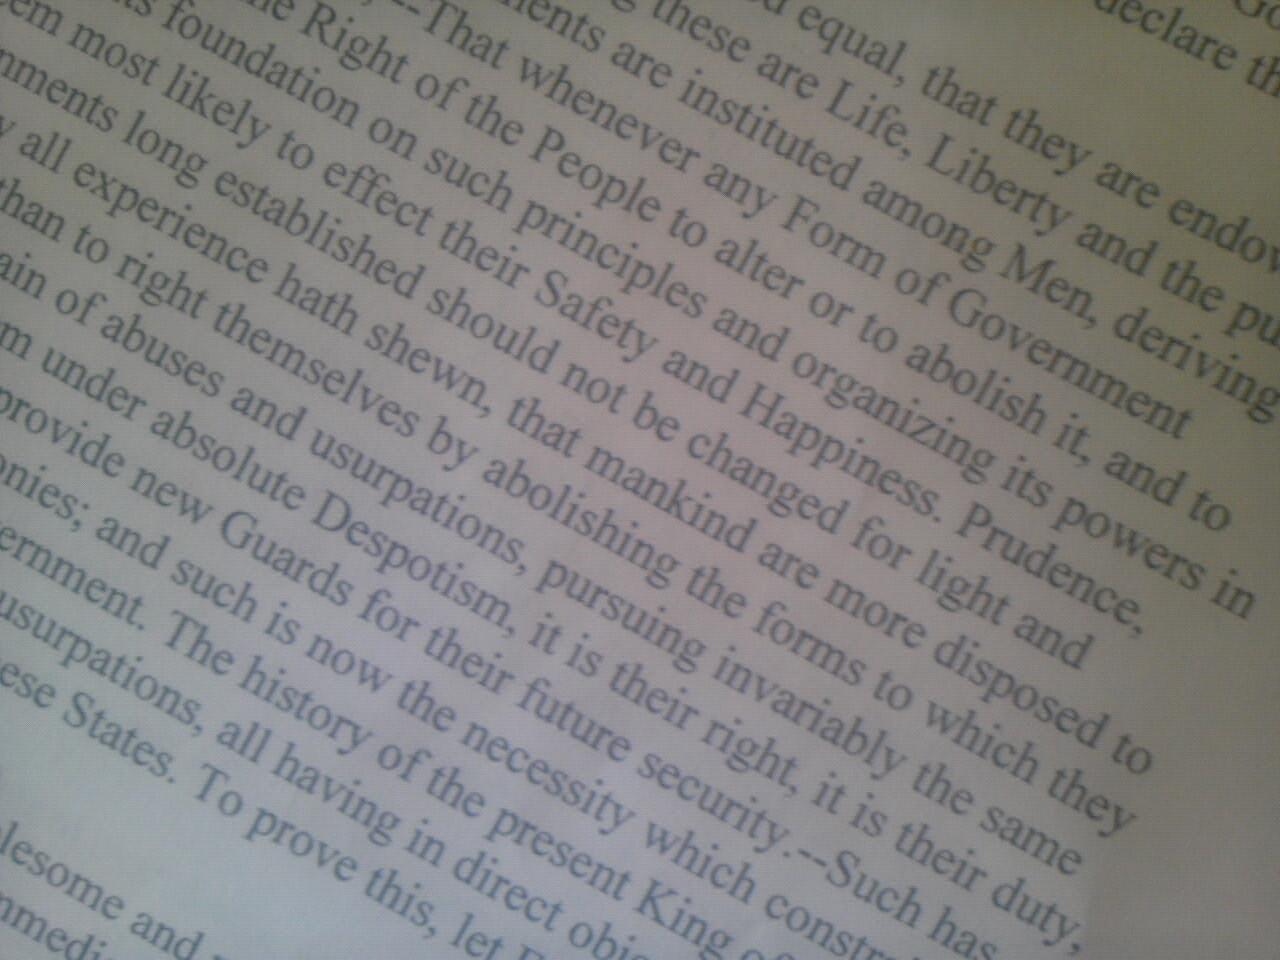
\includegraphics[scale=0.15]{test261.jpg}
\caption{Before Binarization}
\label{noskew}
\end{figure}

\begin{figure}
\center
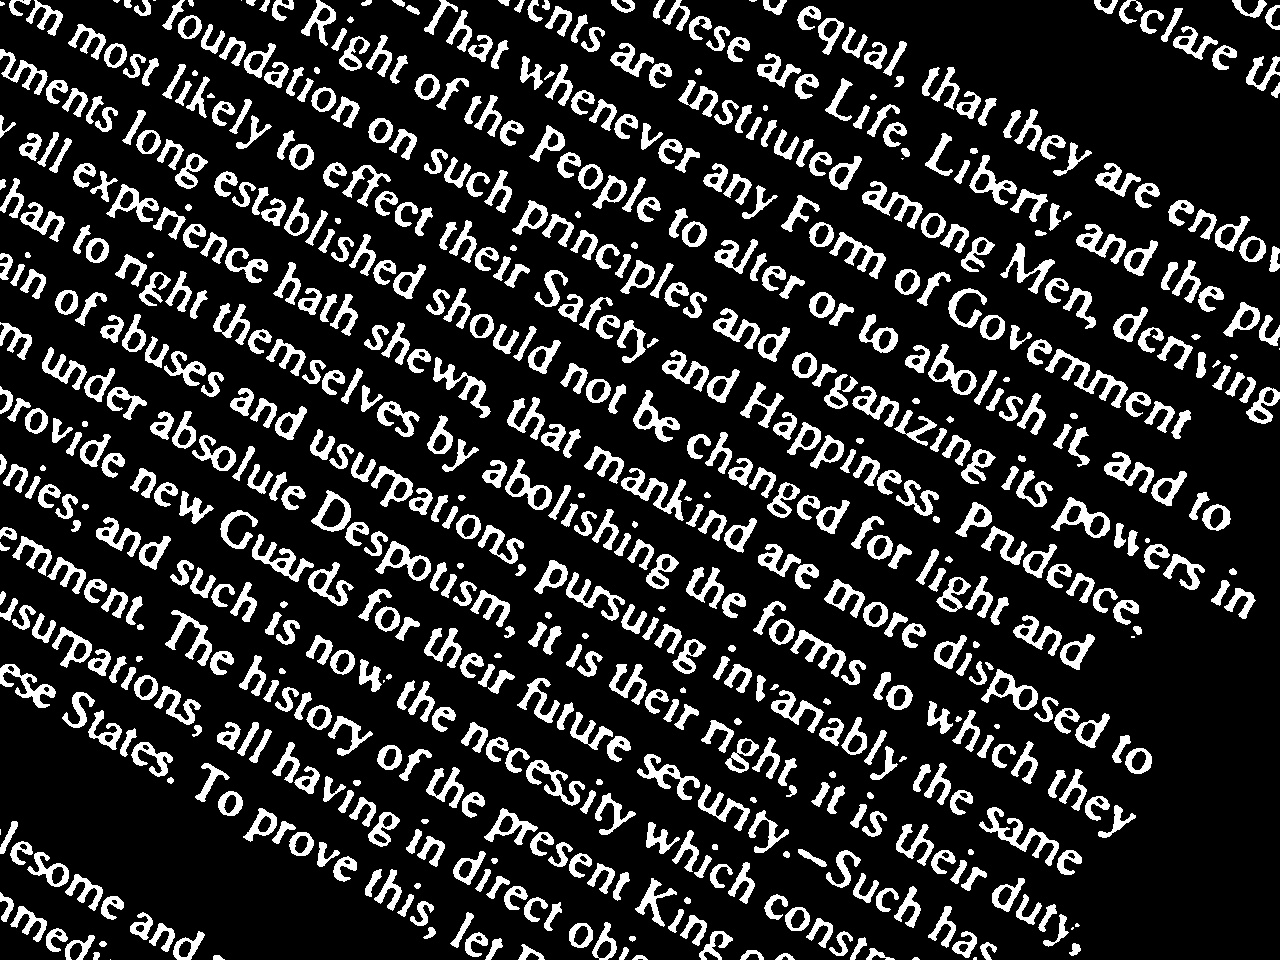
\includegraphics[scale=0.15]{src_image.jpg}
\caption{After Binarization}
\label{noskewbinarized}
\end{figure}

\subsection{De-skew}

Hough transform (OpenCV function HoughLinesP) is used to detect (text) lines in the image.  Then we rotate binarized image by the mean of the rotation angles calculated from each text line, we call OpenCV function getRotationMatrix2D to do it.  We also need to make sure not to cut off corners in the rotation process, therefore we need to pad the binarized image before rotating.  See Figure~\ref{deskewed} for an example of image before and after de-skew.  Notice that Figure~\ref{deskewed} is slightly larger than images above because of padding.

Observing that Tesseract does a decent job for images skewed by less than 5 degrees, we have included logic to bypass de-skew image rotation for such images.  This improves accuracy because image rotation lowers image quality because of interpolation.  By skipping rotation, we essentially preserve more details in the image and therefore boost performance for images with a small skew.

We can see evidence of improvement in Figure~\ref{accuracybyangle}, where 0-degree test cases have better performance than others.  Even though theoretically 0-degree test cases should not be affected by image rotation if the skew is exactly 0 degree, we performed testing by hand-holding the device, which can introduce skew of a few degrees.  Therefore skipping the rotation step can save us from the interpolation effect and boost performance.

\begin{figure}
\center
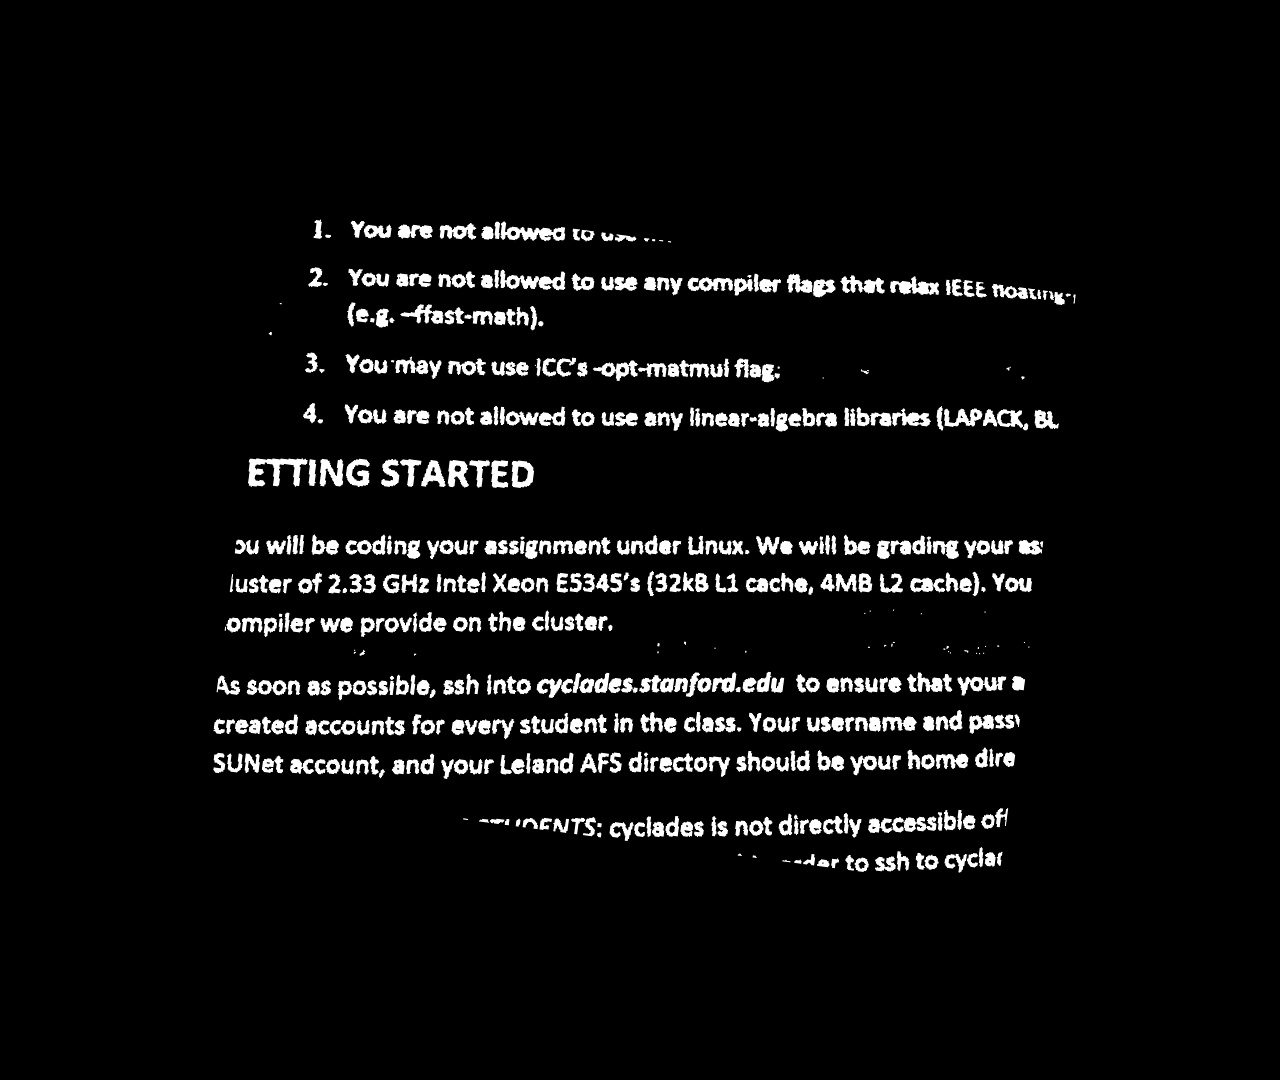
\includegraphics[scale=0.10]{deskewedImage.jpg}
\caption{Binarized And Deskewed}
\label{deskewed}
\end{figure}

\section{Word Recognition}

\subsection{Segmentation By Letter}
The first step of word recognition is to segment the image into rectangles each containing a letter.  Because most letters consists of one connected component in the image, we can draw a contour (OpenCV function findContours and drawContours) around each letter and then find a bounding box of each contour (OpenCV function boundingRect). See Figure~\ref{letterbbox} for an example of each letter surrounded by a rectangular bounding box.

Some letters (for instance, lower case ``i'', ``j'') consists of two connected components, and hence will have two bounding boxes, but it doesn't affect the algorithm since they will get combined in the next step as we combine letter bounding boxes into word bounding boxes.

\begin{figure}
\center
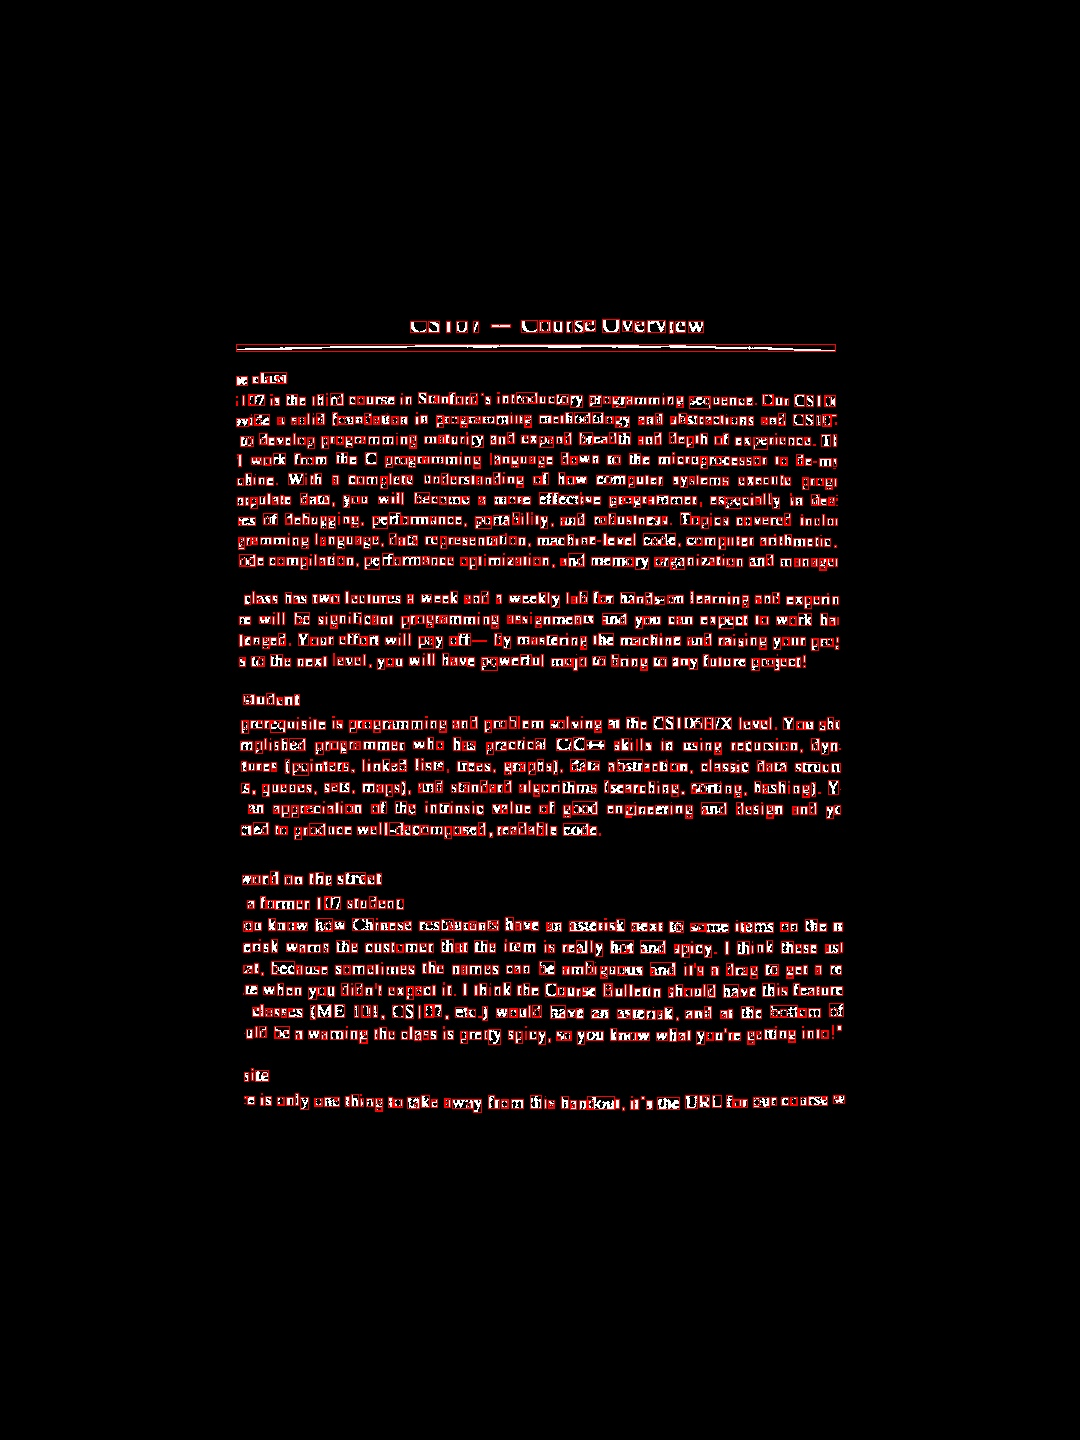
\includegraphics[scale=0.10]{letter_with_bounding_box.jpg}
\caption{Segmentation By Letter}
\label{letterbbox}
\end{figure}

\subsection{Segmentation By Word}

In this step, we need to combine neighbouring letter bounding boxes into a word bounding box, but there is no existing OpenCV functions that performs this task.  We implemented the following functions in C++:

\subsubsection{Find Character Size}
We implemented function findCharSize to estimate the average height and width of each letter (or its bounding box).  This is important because when deciding whether two letter bounding boxes are neighbours, we need to look at the distance between them relative to the average size of bounding boxes, making the decision based on absolute distance only is not accurate.

The implementation was done by creating a map with keys being the areas of the bounding boxes, and the values being the frequencies (i.e. how many bounding boxes has area that equal to the key).  Then we pick the ten most frequent area values and calculate the mean.

The function calculates the values for a few important parameters including:
\begin{itemize}
\item cArea: The mean calculated from the ten most frequent area values.
\item cHeight: An estimate of average height of letters, calculated from $\sqrt{\mbox{cArea}}$ mutiplied by a constant factor 1.1 to take into account that most letters have larger height than width.
\item cWidth: An estimate of average width of letters, calculated from $\sqrt{\mbox{cArea}}$ multiplied by a constant factor 0.75 to take into account that most letters have larger width than height.
\end{itemize}
The constant factors are tuned so that the algorithm works for the majority of test cases.

\subsubsection{Find Neighbour}
We implemented isNeighbour to determine whether two letters are next to each other in the same word.  This is the key logic in determining which letter bounding boxes to merge together into a word bounding box.  Two bounding boxes need to satisfy both conditions below in order to be called neighbours:
\begin{itemize}
\item The x-coordinate of the right edge of box 1 and the x-coordinate of the left edge of box 2 are off by at most $0.32 \times \mbox{cWidth}$ (box 1 is to the left of box 2); or vice versa, the x-coordinate of the left edge of box 1 and the x-coordinate of the right edge of box 2 are off by at most $0.32 \times \mbox{cWidth}$ (box 1 is to the right of box 2).  The factor 0.45 is the parameter that gives the best results after several experiments.
\item  Because different letters have different heights, we decided to use the y-coordinate of the bottom edge to determine whether two boxes are on the same row.  The y-coordinates of the bottom edges of the two boxes needs to be within $0.32 \times \mbox{cHeight}$ of each other.
\item  In addition, we also want to combine the dot in lower case ``i'' and ``j'', therefore we allow the case where the y-coordinates of the top edges are within $0.28 \times \mbox{cHeight}$.
\end{itemize}
The constant factors are tuned so that the algorithm works for the majority of test cases.

See Figure~\ref{wordbbox} for an example of segmentation by word.

\begin{figure}
\center
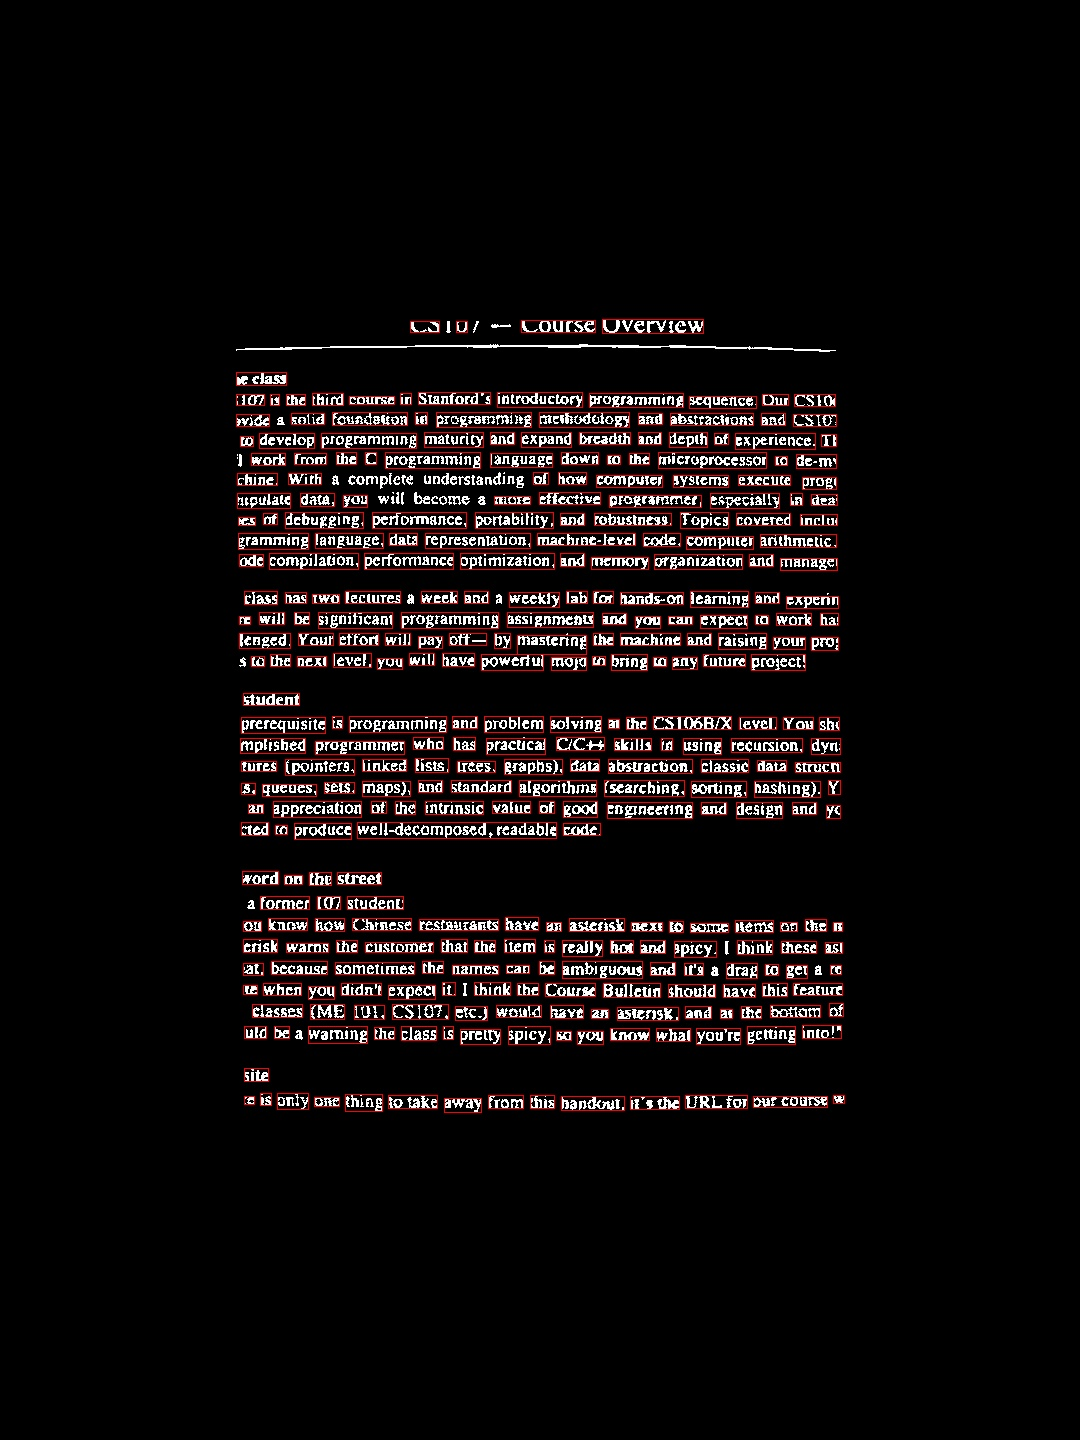
\includegraphics[scale=0.10]{word_with_bounding_box.jpg}
\caption{Segmentation By word}
\label{wordbbox}
\end{figure}

\subsection{Search And Label Matches}
At last we can pass each bounding box (hopefully containing exactly one word at this point) to the Tesseract OCR engine.  Sometimes the image is out of focus or blurry due to vibration, therefore the result from Tesseract is not accurate.  To cope with the imperfection, we label exact matches with a red rectangle, non-exact matches with blue or green rectangles.

Exact or non-exact matches is determined by the ratio between edit distance (or Levenshtein distance) and the length of the keyword.  A ratio of exact zero (or edit distance equal to zero) means that there is an exact match.  A ratio reasonably close to zero means that we have a non-exact match.

Levenshtein distance is defined to be the minimum number of single-letter operations (insertion, deletion or substitution) needed to transform one string into another.  For example, to change ``abcd'' into ``bcda'', one can either change each letter (change the first letter ``a'' to ``b'', the second letter ``b'' to ``c'', the third letter ``c'' to ``d'', the fourth letter ``d'' to ``a'' ), which has a total of four operations, or delete the ``a'' from the beginning of the string and add an ``a'' to the end of it, which has a total of two operations.  Therefore the Levenshtein distance between the two strings is two.  The distance can be calculated between any two strings using recursion.

Finally we draw rectangular boxes of different colors (in order to differentiate between exact matches and close matches) at the coordinates where we find matches, and then overlay the rectangles onto the orginal image.  See Figure~\ref{boxes_overlay} and Figure~\ref{result_image} for illustration of searching and labeling keyword matches.

\begin{figure}
\center
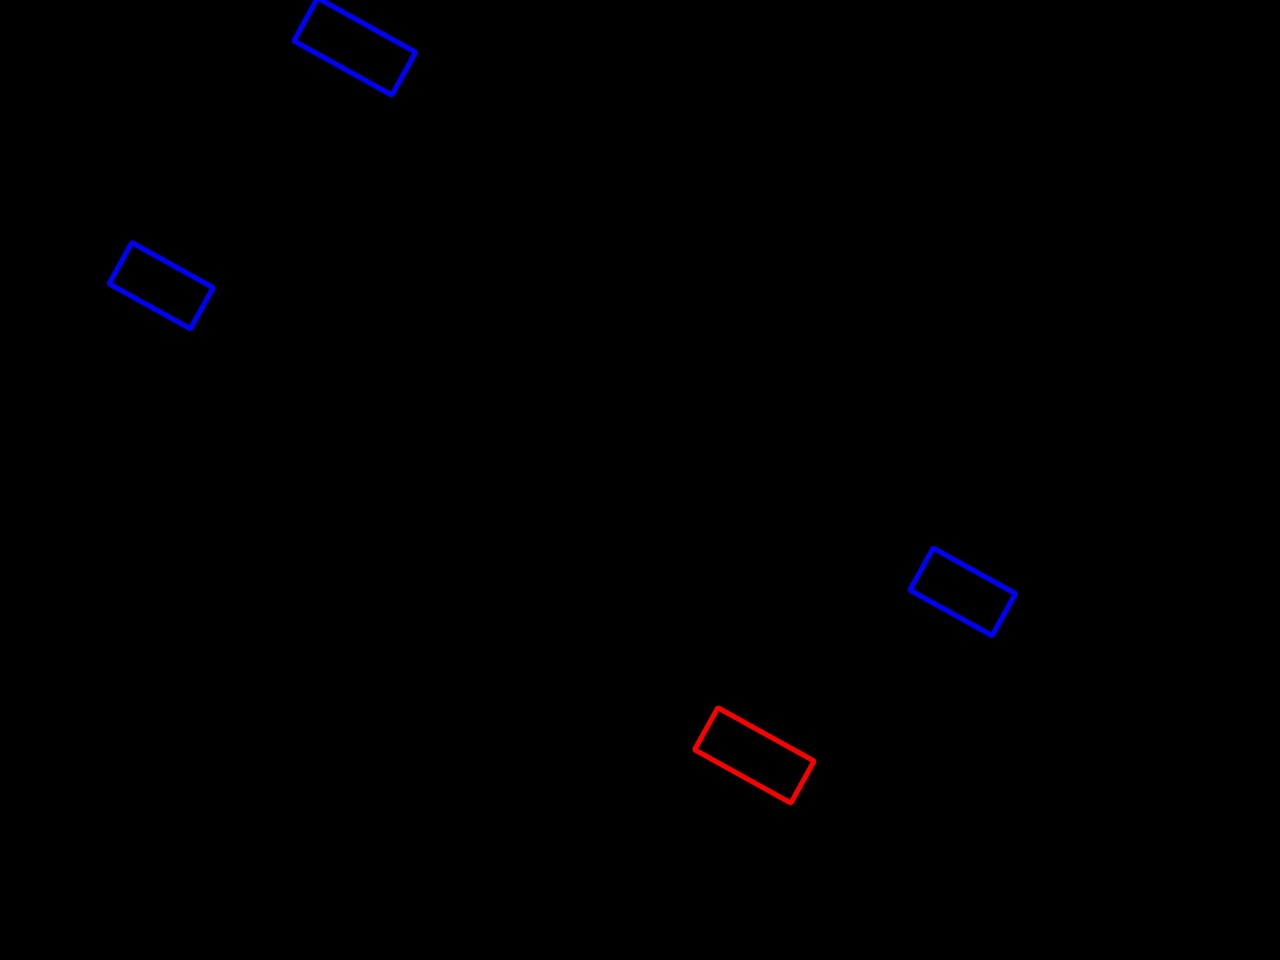
\includegraphics[scale=0.15]{bb_mask_inv_cropped.jpg}
\caption{Highlight Boxes}
\label{boxes_overlay}
\end{figure}

\begin{figure}
\center
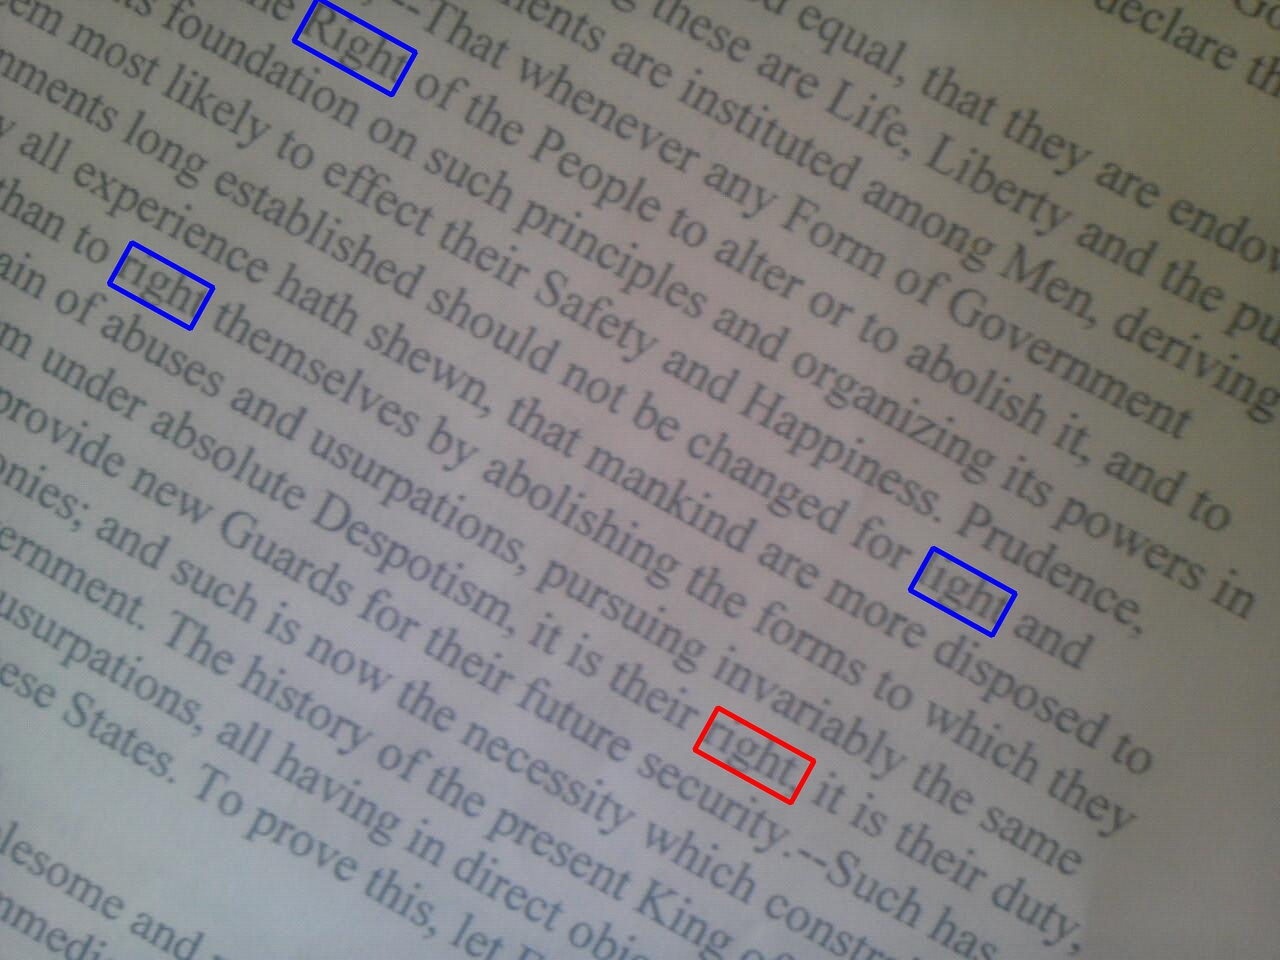
\includegraphics[scale=0.15]{result_image.jpg}
\caption{Result Displayed}
\label{result_image}
\end{figure}


\section{Server Client Connection}

OCR is an extremely computationally intensive operation. To perform this operation using the processors on an outdated smartphone would be impractical. Therefore, we decided to offload OCR and all other image processing operations onto the Stanford servers. The server side consists of two layers. The outer layer is a php script that waits for an http connection. Once the connection is established, the php script receives the image uploaded by the phone along with other parameters and stores them on the afs disk. However the server on which the php script lives does not have the necessary libraries to run OCR and opencv. Therefore, we implemented a backend python script that’s responsible for linking up with the php script and executing the opencv/OCR executable on the Stanford corn server. Once the processing is complete, the php script picks up the output image and streams it back to the phone. 

On the client side, WordHunter has two modes. The first mode, snap mode, takes a picture if the text when the user taps the screen. It then sends the image to the server for processing. After the image is received from the server, the phone will display it on the screen until the user hits the back button to enter a new word.  The second mode, scan mode, continuously cycles through the above mentioned process seamlessly without any user intervention. Instead of displaying the image in the screen however, it will overlay a bounding box on top of the viewfinder to mark the desired word in real time.  Figure~\ref{server_client} illustrates the connection from client side/mobile device to Stanford servers to corn servers.

\begin{figure}
\center
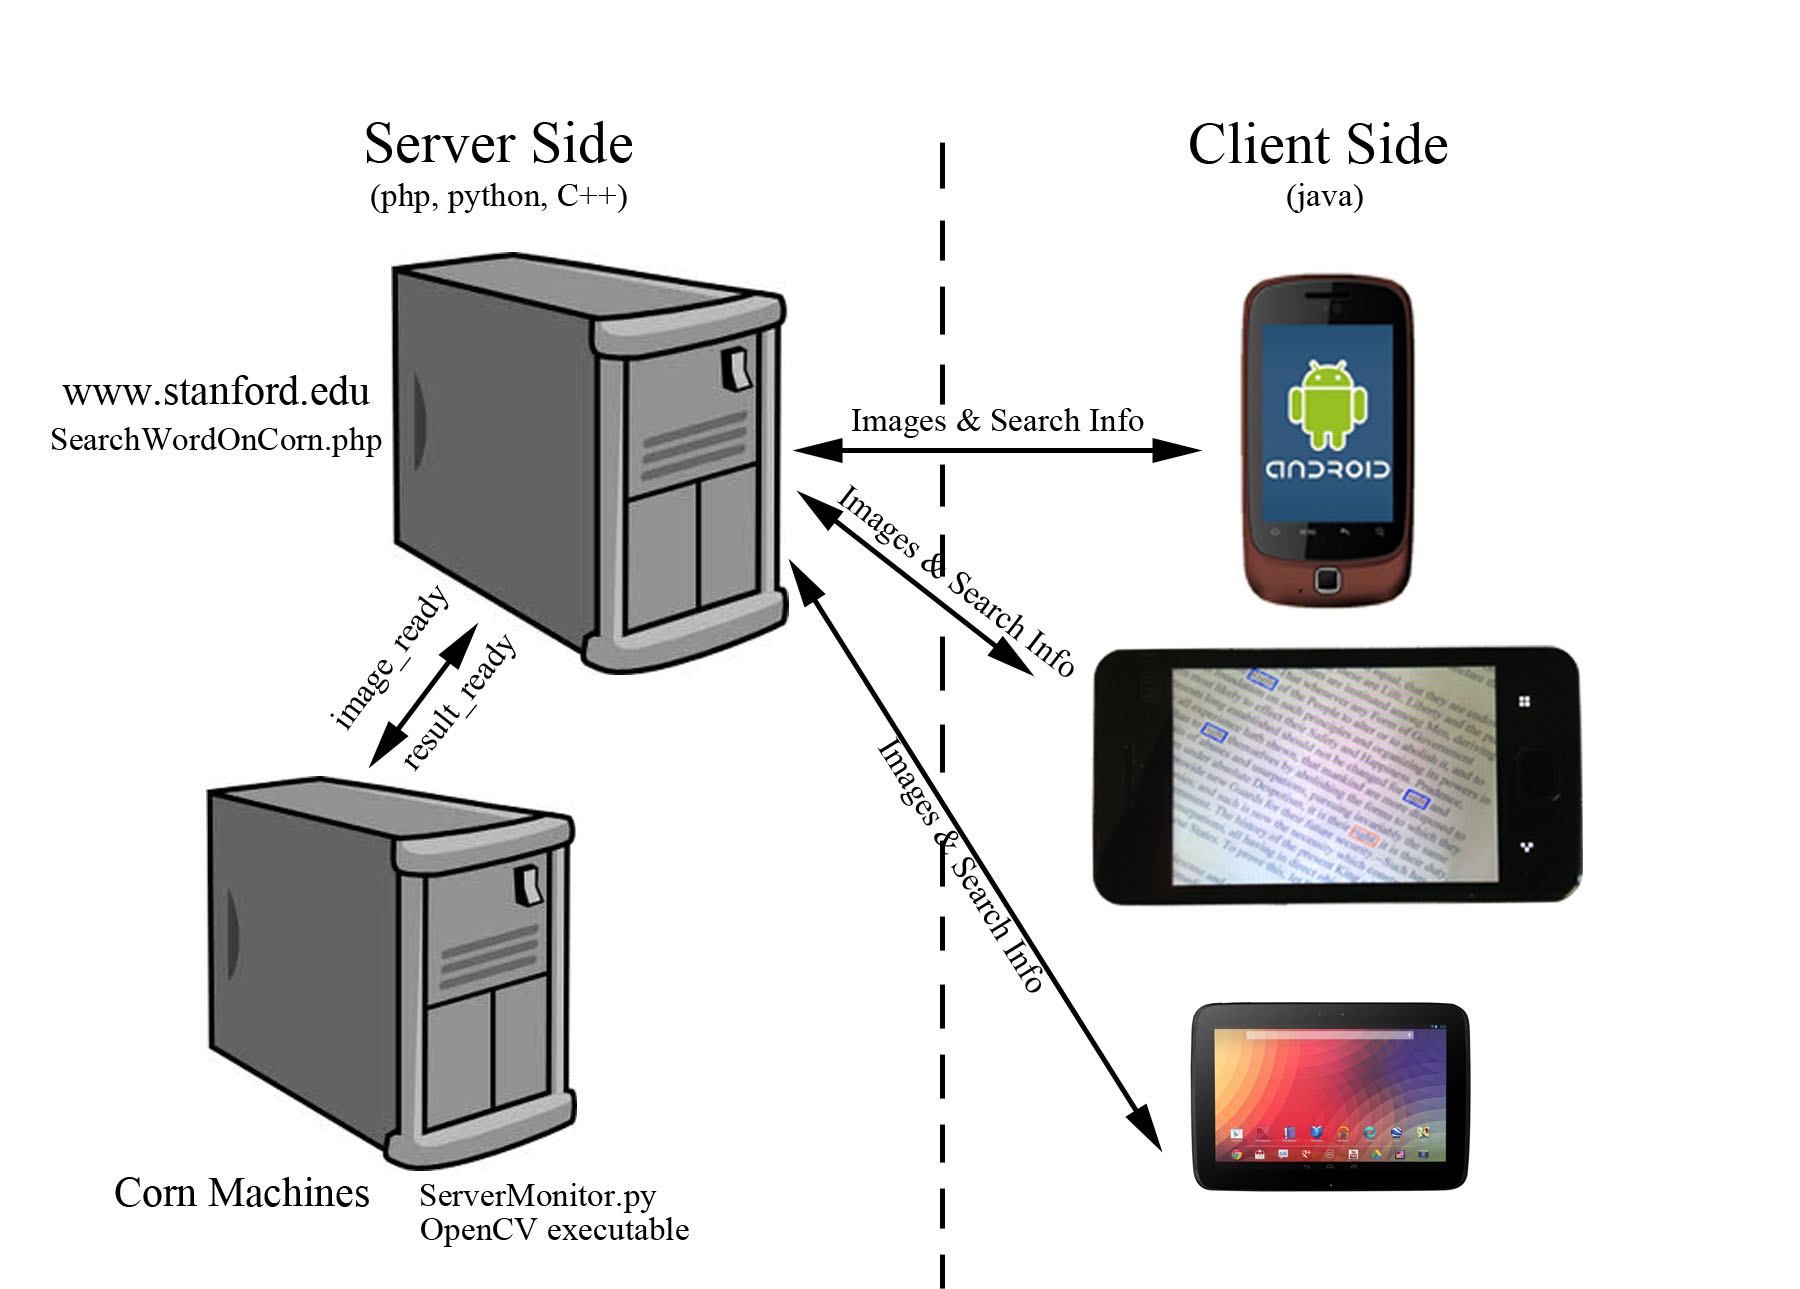
\includegraphics[scale=0.15]{server_client_connection.jpg}
\caption{Server-Client Connection}
\label{server_client}
\end{figure}


\section{Emperical Results}
We tested the keyword recognition rate with more than 100 data points.  The sample space covers different skew angles (0 degree, 15 degrees and 30 degrees), and different word lengths, because we believe that those are the two main factors that can affect performance.    The overall accuracy is 89.7\%, and we have included a breakdown by word length and skew angle (Figure\ref{accuracybylength} and Figure \ref{accuracybyangle}).

From the breakdown by keyword length, we can observe that although accuracy varies for different word lengths, there is no clear trend that performance improves/deteriorates as keyword length increases/decreases, which is desirable.  Variation does exist but it is largely due to the relatively small sample size, we would like to perform most testing if time permits.

From the breakdown by skew angle, notice that there is a slight deterioration in performance due to the skew.  We have investigated this by looking at the intermediate steps/results on the algorithm and concluded that the de-skew algorithm works reasonably well, the deterioration is mostly due to the fact that image rotation lowers the image quality and there is not much we can do about it.  We also noticed that there is very little change in performance from 15-degree skew to 30-degree skew, which is desirable.

We have also noticed (by examining the test input and output images) that results may vary due to uneven line spacing, different fonts, and image quality.  De-focus and blur due to hand shaking account for a large proportion of inaccuracies.

\begin{figure}
\center
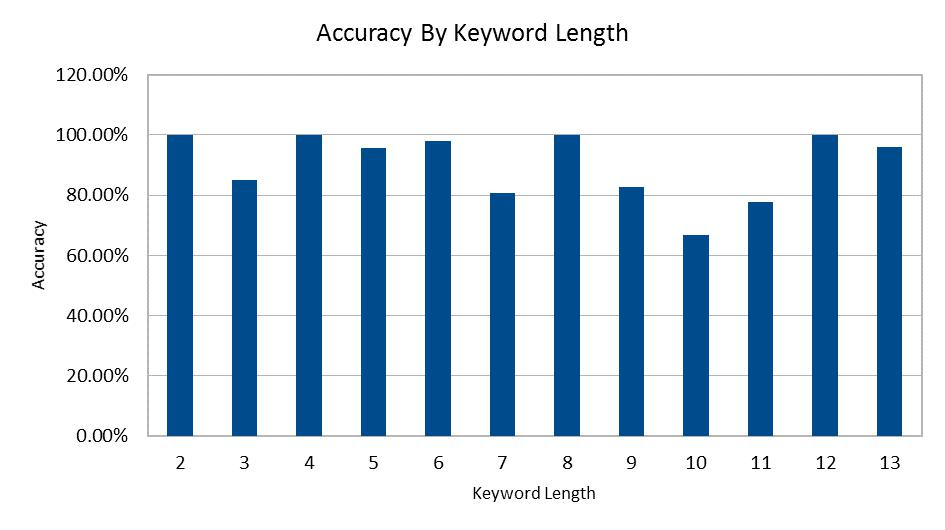
\includegraphics[scale=0.25]{accuracy_by_length.jpg}
\caption{Accuracy By Keyword Length}
\label{accuracybylength}
\end{figure}

\begin{figure}
\center
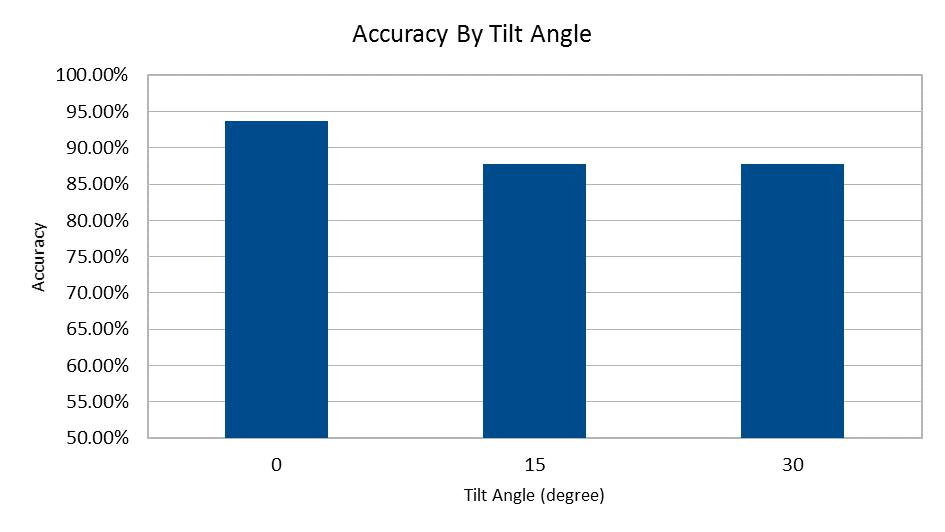
\includegraphics[scale=0.25]{accuracy_by_angle.jpg}
\caption{Accuracy By Skew Angle}
\label{accuracybyangle}
\end{figure}


\section*{Acknowledgment}
We would like to thank David Chen and Sam Tsai for their generous and responsive help on the project.  We would also like to thank Professor Girod for his inspiring lectures.

\section*{Appendix}
The team worked together on the image processing algorithm.  In addition, Yang prototyped the Andriod app and server code, Shuo worked on the app as well as integration, Lingren worked on reporting.

%\begin{thebibliography}{1}
%\bibitem{IEEEhowto:kopka}
%H.~Kopka and P.~W. Daly, \emph{A Guide to \LaTeX}, 3rd~ed.\hskip 1em plus
%  0.5em minus 0.4em\relax Harlow, England: Addison-Wesley, 1999.
%\end{thebibliography}

\end{document}